%% BioMed_Central_Tex_Template_v1.06
%%                                      %
%  bmc_article.tex            ver: 1.06 %
%                                       %

%%IMPORTANT: do not delete the first line of this template
%%It must be present to enable the BMC Submission system to
%%recognise this template!!

%%%%%%%%%%%%%%%%%%%%%%%%%%%%%%%%%%%%%%%%%
%%                                     %%
%%  LaTeX template for BioMed Central  %%
%%     journal article submissions     %%
%%                                     %%
%%          <8 June 2012>              %%
%%                                     %%
%%                                     %%
%%%%%%%%%%%%%%%%%%%%%%%%%%%%%%%%%%%%%%%%%


%%%%%%%%%%%%%%%%%%%%%%%%%%%%%%%%%%%%%%%%%%%%%%%%%%%%%%%%%%%%%%%%%%%%%
%%                                                                 %%
%% For instructions on how to fill out this Tex template           %%
%% document please refer to Readme.html and the instructions for   %%
%% authors page on the biomed central website                      %%
%% http://www.biomedcentral.com/info/authors/                      %%
%%                                                                 %%
%% Please do not use \input{...} to include other tex files.       %%
%% Submit your LaTeX manuscript as one .tex document.              %%
%%                                                                 %%
%% All additional figures and files should be attached             %%
%% separately and not embedded in the \TeX\ document itself.       %%
%%                                                                 %%
%% BioMed Central currently use the MikTex distribution of         %%
%% TeX for Windows) of TeX and LaTeX.  This is available from      %%
%% http://www.miktex.org                                           %%
%%                                                                 %%
%%%%%%%%%%%%%%%%%%%%%%%%%%%%%%%%%%%%%%%%%%%%%%%%%%%%%%%%%%%%%%%%%%%%%

%%% additional documentclass options:
%  [doublespacing]
%  [linenumbers]   - put the line numbers on margins

%%% loading packages, author definitions

\documentclass[twocolumn]{bmcart}% uncomment this for twocolumn layout and comment line below
%\documentclass{bmcart}

%%% Load packages
%\usepackage{amsthm,amsmath}
%\RequirePackage{natbib}
%\RequirePackage[authoryear]{natbib}% uncomment this for author-year bibliography
%\RequirePackage{hyperref}
\usepackage{natbib}
\usepackage[utf8]{inputenc} %unicode support
\usepackage{array}
\usepackage{tipa}
\usepackage{fixltx2e}
\usepackage{algorithm}
\usepackage{enumerate}
\usepackage{graphicx}% http://ctan.org/pkg/graphicx
%\usepackage{pdfpages}
%\usepackage[applemac]{inputenc} %applemac support if unicode package fails
%\usepackage[latin1]{inputenc} %UNIX support if unicode package fails


%%%%%%%%%%%%%%%%%%%%%%%%%%%%%%%%%%%%%%%%%%%%%%%%%
%%                                             %%
%%  If you wish to display your graphics for   %%
%%  your own use using includegraphic or       %%
%%  includegraphics, then comment out the      %%
%%  following two lines of code.               %%
%%  NB: These line *must* be included when     %%
%%  submitting to BMC.                         %%
%%  All figure files must be submitted as      %%
%%  separate graphics through the BMC          %%
%%  submission process, not included in the    %%
%%  submitted article.                         %%
%%                                             %%
%%%%%%%%%%%%%%%%%%%%%%%%%%%%%%%%%%%%%%%%%%%%%%%%%


%\def\includegraphic{}
%\def\includegraphics{}



%%% Put your definitions there:
\startlocaldefs
\newcommand{\specialcell}[2][c]{%
  \begin{tabular}[#1]{@{}c@{}}#2\end{tabular}}
\endlocaldefs


%%% Begin ...
\begin{document}

%%% Start of article front matter
\begin{frontmatter}
\thispagestyle{plain}
\begin{fmbox}
\dochead{Research}
%%%%%%%%%%%%%%%%%%%%%%%%%%%%%%%%%%%%%%%%%%%%%%
%%                                          %%
%% Enter the title of your article here     %%
%%                                          %%
%%%%%%%%%%%%%%%%%%%%%%%%%%%%%%%%%%%%%%%%%%%%%%

\title{Listener: A prototype system for automatic speech recognition and evaluation of
Brazilian-accented English}

%%%%%%%%%%%%%%%%%%%%%%%%%%%%%%%%%%%%%%%%%%%%%%
%%                                          %%
%% Enter the authors here                   %%
%%                                          %%
%% Specify information, if available,       %%
%% in the form:                             %%
%%   <key>={<id1>,<id2>}                    %%
%%   <key>=                                 %%
%% Comment or delete the keys which are     %%
%% not used. Repeat \author command as much %%
%% as required.                             %%
%%                                          %%
%%%%%%%%%%%%%%%%%%%%%%%%%%%%%%%%%%%%%%%%%%%%%%

\author[
   addressref={aff1},                   % id's of addresses, e.g. {aff1,aff2}
   corref={aff1},                       % id of corresponding address, if any
   %noteref={n1},                        % id's of article notes, if any
   email={gustavoauma@gmail.com}   % email address
]{\inits{GA}\fnm{Gustavo A} \snm{Mendon\c{c}a}}
\author[
   addressref={aff1},
   corref={aff1},
   email={sandram@icmc.usp.br}
]{\inits{SM}\fnm{Sandra M} \snm{Aluisio}}

%%%%%%%%%%%%%%%%%%%%%%%%%%%%%%%%%%%%%%%%%%%%%%
%%                                          %%
%% Enter the authors' addresses here        %%
%%                                          %%
%% Repeat \address commands as much as      %%
%% required.                                %%
%%                                          %%
%%%%%%%%%%%%%%%%%%%%%%%%%%%%%%%%%%%%%%%%%%%%%%

\address[id=aff1]{%                           % unique id
  \orgname{Instituto de Ci\^encias Matem\'aticas e de Computa\c{c}\~ao}, % university, etc
  \street{Universidade de S\~ao Paulo},                     %
  %\postcode{8045}                                % post or zip code
  \city{S\~ao Carlos -- SP},                              % city
  \cny{Brazil}                                    % country
}

%%%%%%%%%%%%%%%%%%%%%%%%%%%%%%%%%%%%%%%%%%%%%%
%%                                          %%
%% Enter short notes here                   %%
%%                                          %%
%% Short notes will be after addresses      %%
%% on first page.                           %%
%%                                          %%
%%%%%%%%%%%%%%%%%%%%%%%%%%%%%%%%%%%%%%%%%%%%%%

\begin{artnotes}
%\note{Sample of title note}     % note to the article
%\note[id=n1]{Equal contributor} % note, connected to author
\end{artnotes}

\end{fmbox}% comment this for two column layout

%%%%%%%%%%%%%%%%%%%%%%%%%%%%%%%%%%%%%%%%%%%%%%
%%                                          %%
%% The Abstract begins here                 %%
%%                                          %%
%% Please refer to the Instructions for     %%
%% authors on http://www.biomedcentral.com  %%
%% and include the section headings         %%
%% accordingly for your article type.       %%
%%                                          %%
%%%%%%%%%%%%%%%%%%%%%%%%%%%%%%%%%%%%%%%%%%%%%%

\begin{abstractbox}

\begin{abstract} % abstract
Recent surveys have shown that Brazil is among the countries with the lowest knowledge of the English language. Considering that English is the current lingua franca, any effort that seeks to improve such knowledge is worthwhile. This paper presents a project aimed at being a primary step towards developing a pronunciation assessment system for Brazilian-accented English. Lately, with increased computing power and improved speech recognition, research on automated pronunciation error detection and pronunciation assessment has gained attention. The prototype developed herein, called Listener, is based on speech recognition and comprises three modules: (i) a pronunciation model; (ii) an acoustic model; and (iii) a context free grammar. Pronunciation variants were added manually to a lexicon of 1,841 words through transcription rules. The acoustic model was trained on a combined model, which is fed with data from English, Portuguese and Brazilian-accented English. Context free grammars were used to allow forced-alignment. The prototype achieved a true positive rate of 0.90 on detecting mispronunciations in clean speech. However, in noisy data, the performance was severely damaged, being as low as 0.57 for isolated words or 0.31 for words+sentences.
\end{abstract}

%%%%%%%%%%%%%%%%%%%%%%%%%%%%%%%%%%%%%%%%%%%%%%
%%                                          %%
%% The keywords begin here                  %%
%%                                          %%
%% Put each keyword in separate \kwd{}.     %%
%%                                          %%
%%%%%%%%%%%%%%%%%%%%%%%%%%%%%%%%%%%%%%%%%%%%%%

\begin{keyword}
\kwd{pronunciation training}
\kwd{non-native speech recognition}
\kwd{natural language processing}
\end{keyword}

% MSC classifications codes, if any
%\begin{keyword}[class=AMS]
%\kwd[Primary ]{}
%\kwd{}
%\kwd[; secondary ]{}
%\end{keyword}

\end{abstractbox}
%
%\end{fmbox}% uncomment this for twcolumn layout

\end{frontmatter}

%%%%%%%%%%%%%%%%%%%%%%%%%%%%%%%%%%%%%%%%%%%%%%
%%                                          %%
%% The Main Body begins here                %%
%%                                          %%
%% Please refer to the instructions for     %%
%% authors on:                              %%
%% http://www.biomedcentral.com/info/authors%%
%% and include the section headings         %%
%% accordingly for your article type.       %%
%%                                          %%
%% See the Results and Discussion section   %%
%% for details on how to create sub-sections%%
%%                                          %%
%% use \cite{...} to cite references        %%
%%  \cite{koon} and                         %%
%%  \cite{oreg,khar,zvai,xjon,schn,pond}    %%
%%  \nocite{smith,marg,hunn,advi,koha,mouse}%%
%%                                          %%
%%%%%%%%%%%%%%%%%%%%%%%%%%%%%%%%%%%%%%%%%%%%%%

%%%%%%%%%%%%%%%%%%%%%%%%% start of article main body
% <put your article body there>

%%%%%%%%%%%%%%%%
%% Background %%
%%

\pagestyle{plain}
%************************************************
\section{Introduction}
%************************************************
According to the International Monetary Found (IMF) \cite{IMF2015}, in 2015, Brazil was the seventh largest economy in the world with a GDP of US\$ 2.34 trillions. A survey by The Economist (2013) says that, since 2009, the growth of BRICS accounts for 55\% of the entire world economy growth. The current economic scenario is extremely favourable for Brazil to increase its global influence; however with regard to the ability to communicate globally, Brazil occupies a much more modest position. 

In 2015, Brazil ranked 41\textsuperscript{st} out of 70 countries in the English Proficiency Index (EF-EPI) \cite{EF2015}, classified among countries with low English proficiency, with 51.05 points. Scandinavian countries led the very high proficiency rankings, with Sweden (70.94) in the first position, Denmark (70.05) in third the spot and Norway (67.83) in fourth. Brazil performance was close to several other Latin America countries, such as Peru (52.46), Chile (51.88), Ecuador (51.67), Uruguay (50.25) and Colombia (46.54). The only exception in Latin America was Argentina that, despite the recent great depression, was ranked 15\textsuperscript{th}, being classified as high proficiency, with a score of 60.26.

The EF-EPI bands are aligned to the Common European Framework of Reference for Languages (CEFR) in the following way: the very high proficiency band corresponds to CEFR level B2; very low proficiency to A2; high, moderate and low proficiency bands to B1 with different punctuations. In case, Brazil's low proficiency rank is analogous to the CEFR level B1, that describes an independent language user with the intermediate communication skills (see Table ~\ref{tab:cefr-levels}.

\renewcommand{\arraystretch}{1.2}
\begin{table}[!htpb]
\newcolumntype{A}{>{\arraybackslash}p{.02\textwidth}}
\newcolumntype{B}{>{\arraybackslash}p{.42\textwidth}}
\caption{CEFR reference level description for B1.}
\small
\setlength\tabcolsep{1.8pt}
\begin{center}
\begin{tabular}[t]{AB}
\hline
\textbf{\#} & \textbf{\centering Communication skills} \\ \hline
1 & Can understand the main points of clear standard input on familiar matters regularly encountered in work, school, leisure, etc. \\ 
2 & Can deal with most situations likely to arise while traveling in an area where the language is spoken. \\ 
3 & Can produce simple connected text on topics that are familiar or of personal interest. \\
4 & Can describe experiences and events, dreams, hopes and ambitions and briefly give reasons and explanations for opinions and plans. \\ \hline
\end{tabular}
\end{center}
\label{tab:cefr-levels}
\end{table}
\renewcommand{\arraystretch}{1.0}

As one might notice,  the B1 level describes an individual who is usually able to understand familiar matters, deal with traveling situations, describe personal experiences and plans, and produce simple texts about subjects of personal interest. Needless to say, this is a very restricted communicative competence, which limits English usage primarily to the personal domain. 

With respect of Business English proficiency, Brazil performance is even more concerning. On the 
Business English Index (BEI) of 2013 \cite{BEI2013}, Brazil reached the 71\textsuperscript{st} position out of 77 countries analyzed. We attained a score of 3.27 points, in a scale from 1 to 10, being placed at the ``Beginner'' range, the lowest range considered by the index. We were close to countries such as El Salvador (3.24), Saudi Arabia (3.14) and Honduras (2.92) which up until recently had experienced civil wars or dictatorship governments. BEI describes individuals at the beginner level as those who ``can read and communicate using only simple questions and statements, but can't communicate and understand basic business information during phone calls''. Again, we can see that this is a very limited linguistic competence, that would not allow one not even to perform the most elementary day-to-day task in a company or industry work environment.

Given this scenario, it is clear that we urgently need to improve English language proficiency among Brazilians. This project seeks to be an initial step towards this direction. We developed a prototype system for automatic speech recognition and evaluation of Brazilian-accented English, called \emph{Listener}, which is capable of recognizing utterances in Brazilian-accented English and identifying which are the mispronunciations. The system was designed especially for graduate students who want to improve their pronunciation skills. The interest in this group is due to the fact that graduate students often need to speak English in order to publicize their research, for instance, by attending conferences or giving lectures. The system is based on an Automatic Speech Recognition system which makes use of forced alignment, \emph{HMM}/\emph{GMM} acoustic models, context free grammars and multipronunciation dictionaries\footnote{All files, resources and scripts developed are available at the project website: http://nilc.icmc.usp.br/listener. Due to copyright reasons, the corpora used for training the acoustic models cannot be made available. }.

This paper is structured as follows. Section ~\ref{sec:speech-recognition} presents some fundamental concepts in speech recognition. Section ~\ref{method} discusses the materials and methods, with an overview of pronunciation models, acoustic models, as well as context free grammars. Results are shown in Section ~\ref{results}. Finally, in Section ~\ref{conclusion} we present the overal conclusions, discuss the work limitations and present some future work.

%*****************************************
\section{Automatic Speech Recognition}\label{sec:speech-recognition}
%*****************************************

Automatic Speech Recognition (ASR) can be defined as the task of converting spoken language into readable text by computers in real-time \cite{Huang2001}. 

Speech is certainly the most natural human way of communication. Allowing people to interact with their gadgets through voice may greatly improve the user-experience, especially in a world which is becoming more and more mobile-oriented. Currently, ASR is present in many widely-used applications, such as personal assistants, speech-to-text processing, domotics, call routing, etc. \cite{Candeias2014}

All state-of-the-art paradigms in ASR are stochastic and they basically try to solve one single equation, which is called the fundamental equation of \emph{ASR}. It can be described as follows. Let $O$ be a sequence of observable acoustic feature vectors and $W$ be a word sequence, the most likely word sequence $W*$ is given by:

\begin{equation}{\label{eq:fund-asr}}
W*= \arg\max_{W}P(W|O)
\end{equation}

To solve this equation straightforwadly, one would require a discriminative model
capable of estimating the the probability of $W$ directly from a set of observations $O$ \cite{Gales2008}.
If we apply the Bayes' Theorem we obtain the following equivalent equation:

\begin{equation}
W*= \arg\max_{W}\frac{P(O|W)P(W)}{P(O)}
\end{equation}

which is suitable for a generative model. For a single audio input, the probability of the observable acoustic feature vectors $P(O)$ is a constant and, therefore, might be discarded, in such way that we end up with:

\begin{equation}
W*= \arg\max_{W}P(O|W)P(W)
\end{equation}

$P(O|W)$ is the conditional probability of an observable acoustic feature vector given a word sequence, is calculated by an acoustic model. In turn, $P(W)$, the \emph{a priori} probability of words is reckoned by a language model or through grammars. 

\begin{figure*}[!ht]

        {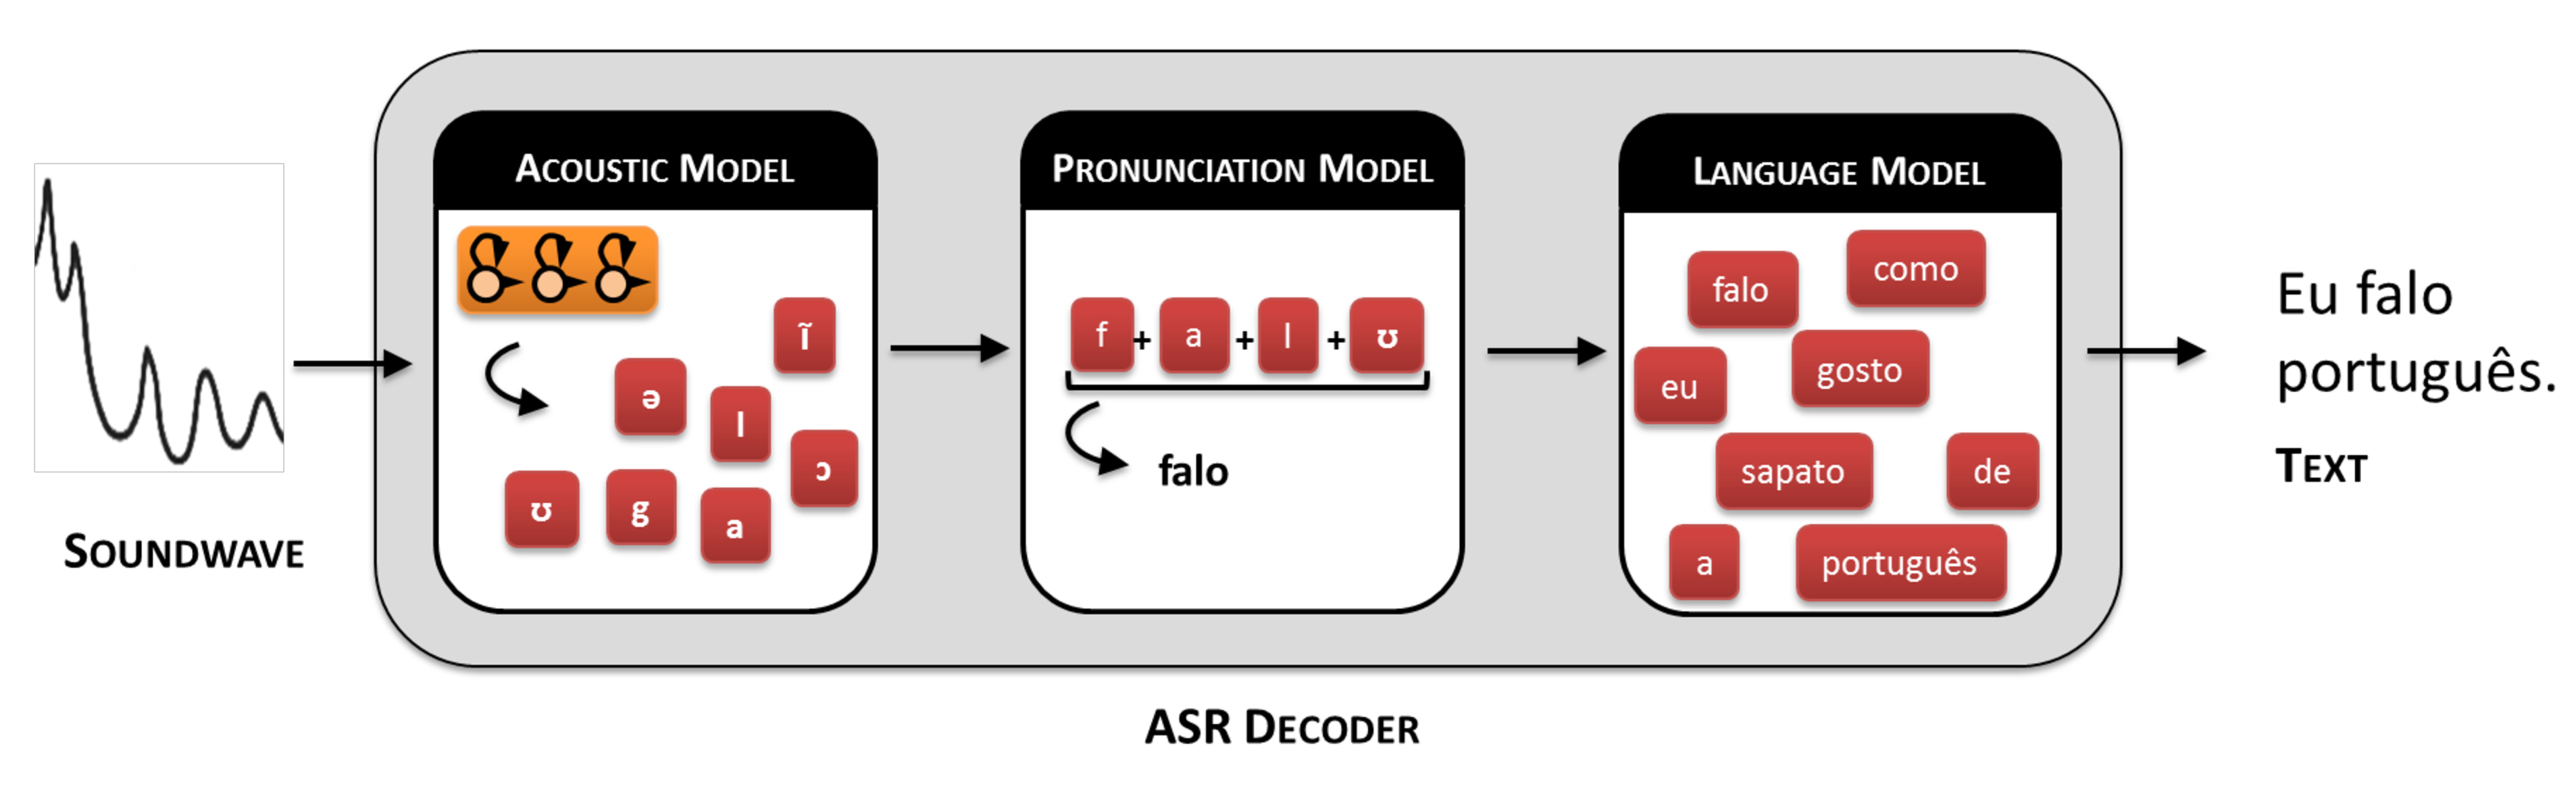
\includegraphics[width=1.7\linewidth]{gfx/asr-architecture.pdf}}
        \caption{Architecture of a continuous speech recognition system. Note: in the Listener prototype, the language model is replaced by a context free grammar.}
        \label{fig:asr-gen-architecture}
\end{figure*}

Figure \ref{fig:asr-gen-architecture} illustrates the basic architecture of an ASR system. The acoustic model processes the acoustic signal of the speech. This model does so in order for it to infer what sound segments comprise the speech, usually by means of using phones or triphones. In HMM-based recognisers, the task of processing the acoustc signal is carried out estimating the most likely observed acoustic states as well as their transition probabilities. On the other hand, the pronunciation model provides us with the correspondence between phones and words sequences in the language. In the example, such model maps on the sequence of phones [falU] in the word "falo". The language model, in its turn, estimates the ordering of the most likely words in the language; in the prototype described herein, this step is performed by the grammar, to parse the many pronunciation variants.

%*****************************************
\section{Materials and Methods}\label{method}
%*****************************************

\subsection{Architecture of Listener}\label{architecture}
The prototype of the Listener system has three modules: (i) a pronunciation model; (ii) an acoustic model; and (iii) a context free grammar. In the following subsections each of these modules will be discussed in detail.

\subsection{Pronunciation Model}\label{pron_model}

Pronunciation models are lexica with words and their corresponding phonetic transcriptions, according to a given convention. In other words, pronunciation models have the role of linking phones from the acoustic model to words defined in the language model. For speech recognition purposes, phonetic a like ARPAbet or SAMPA are often employed to avoid problems with data formatting or encoding. In ARPAbet, phones are converted into sequences of ASCII characters, in such a way that a word like ``speech'' [\textipa{'spi:tS}] becomes [s p iy1 ch] \cite{CMUDict2008}.

For non-native speech recognition, multipronunciation dictionaries are often employed in order to address phenomena of negative-transference from the L1 to L2 \cite{Strik2001}. These dictionaries are a type of pronunciation model where pronunciation variants are explicitly added to the lexicon of the ASR \cite{Strik2001}. For building the pronunciation model for Listener, the literature on pronunciation training was analyzed and transformation rules were defined based on the most common mispronunciations among Brazilians. The pronunciation model was inspired by several works for pronunciation training, focused on Brazilian-accented English \citep{Zimmer2004, Zimmer2009, Cristofaro2015}. In total, we gathered 13 mispronunciation patterns for Listener, the full list with examples can be found in Table ~\ref{tab-mispronunciations}.

\renewcommand{\arraystretch}{1.2}% Tighter
\begin{table}[!ht]
\caption[Mispronunciation types.]{Mispronunciation types selected for the prototype system with examples of the expected pronunciation and the one with negative transfer from L1 to L2.}\label{tab-mispronunciations}
\setlength\tabcolsep{1.8pt}
\small
\begin{tabular}{lllll}
\hline
\textbf{\#} & \textbf{Description} & \textbf{Example} & \textbf{Expect.} & \textbf{Mispron.} \\  \hline
1 & Initial epenthesis & school & [\textipa{sku:l}] & [\textipa{isku:l}] \\
2 & Coda epenthesis & dog & [\textipa{dA:g}] & [\textipa{dA:gi}] \\
3 & Terminal devoicing & does & [\textipa{d2z}] & [\textipa{d2s}] \\
4 & Th-fronting & think & [\textipa{TINk}] & [\textipa{fINk}] \\
5 & Palatalization & teen & [\textipa{t\super hi:n}] & [\textipa{tSi:n}] \\
6 & Deaspiration in plosives & tea & [\textipa{t\super hi:}] & [\textipa{ti:}] \\
7 & Vocalization of laterals & well & [\textipa{wEl}] & [\textipa{wew}] \\
8 & Vocalization of nasals & beam & [\textipa{bi:m}] & [\textipa{b\~i}] \\
9 & Velar paragoge & wing & [\textipa{wIN}] & [\textipa{wINg}] \\ 
10 & Consonantal change & think & [\textipa{TINk}] & [\textipa{fINk}] \\
11 & Vowel change & put & [\textipa{p\super hUt}] & [\textipa{p\super h2t}] \\ 
12 & General deletion & foot & [\textipa{fUt}] & [\textipa{fU}] \\
13 & General insertion & work & [\textipa{w3:rk}] & [\textipa{w3:rks}] \\ \hline
\end{tabular}
\end{table}
\renewcommand{\arraystretch}{1.0}

All linguistic contexts described by Zimmer \cite{Zimmer2004} were converted into transcription rules in order to generate the variants for the pronunciation dictionary. The full list of rules can be found in the project's website. A sample of these rules can be found in Figure ~\ref{pseudocode-rules}. These transcription rules are then applied to a base dictionary in order to append it with new pronunciation variants.

\begin{figure}[!ht]
  \caption{\csentence{Building the pronunciation model.}
      Pseudocode with the rules for generating pronunciation variants (sample).}
      \label{pseudocode-rules}
\small
\begin{tabular}{l} \hline
\small
\\ 
\textbf{\# Initial epenthesis} \\
if [s p] in initial position $\rightarrow$ [iy s p] \# sport \\
if [s t] in initial position $\rightarrow$ [iy s t] \# start \\
if [s k] in initial position $\rightarrow$ [iy s k] \# skate \\
if [s m] in initial position $\rightarrow$ [iy s m] \# small \\
if [s n] in initial position $\rightarrow$ [iy s n] \# snake \\
 ...  \\
\textbf{\# Coda epenthesis} \\
if [p] in final position $\rightarrow$ [p ih] \# stop \\
if [b] in final position $\rightarrow$ [b ih] \# bob \\
if [t] in final position $\rightarrow$ [t ih] \# boat \\
if [d] in final position $\rightarrow$ [d ih] \# and \\ 
if [k] in final position $\rightarrow$ [k ih] \# book \\
if [g] in final position $\rightarrow$ [g ih] \# dog \\
 ...  \\
if [m] and ortho ends in $<$me$>$ $\rightarrow$ [m ih] \# time \\
if [s] and ortho ends in $<$ce$>$ $\rightarrow$ [s ih] \# nice \\
 ...  \\
\textbf{\# Th-fronting} \\
if [th] $\rightarrow$ [f] \# think \\
if [th] $\rightarrow$ [s] \# think \\
if [th] $\rightarrow$ [t] \# think \\
... \\
\textbf{\# Palatalization} \\
if [t iy] $\rightarrow$ [ch iy] \# teen \\
if [t ih] $\rightarrow$ [ch iy] \# poetic \\
 ... \\
\textbf{\# Vocalization of nasal consonants} \\
if [iy m] in final position $\rightarrow$ [im] \# him \\
if [ae n] in final position $\rightarrow$ [em] \# can \\
... \\
\end{tabular}
\end{figure}

It is worth noticing that, in terms of context, there is often overlapping among rules. For instance, in a word like ``think'' [th ih ng k], there is a rule for converting [th] into [f], another one for converting it into [s], or [t], etc. There are even rules which create context for other ones to apply, for instance, in ``boat'' [b ow t], if epenthesis takes place, generating [b ow t ih], then [t] could undergo consonantal change/palatalization, thus producing [b ow ch ih].

To make sure that all pronunciation variants are generated, the rules are run inside a while loop, which iterates over each word in the base dictionary generating and adding these new pronunciation to the dictionary; and the loop only stops when there are no new variants.

For the pilot system of Listener, we used the CMUdict \cite{CMUDict2008} as a base dictionary, which contains over 134,000 entries and their pronunciations in American English. However, in the test sets for Listener there are 1,841 unique words, therefore only these were considered in this experiment. These transcription rules were run over these 1,841 unique words and 8,457 new pronunciation variants were generated (totalling 10,298 entries in the final dictionary). In such a way, the average pronunciation per word is 5.6. 

\subsection{Acoustic Model}

Acoustic Models (AM) are used within speech recognition to map the acoustic parameters of into phonemes.  AMs are estimated through supervised training over a transcribed speech corpus -- often with the Forward-Backward algorithm by modeling phones via Hidden Markov Models (HMM) \cite{Rabiner1989}. Markov models are very suitable for the statistical description of symbol and state sequences \cite{Fink2014}. Within Markov processes, systems are assumed to be memoryless, that is, the conditional probability of future states is only dependent on the present state. To put it another way, the current state does not depend upon the 
sequence of events that preceded it. Hidden Markov Models (HMM) are just a special type of Markov processes which contain hidden states.

HMMs are the most widespread models used in ASR \cite{Juang2005}. They can be formally described as a 5-tuple $\lambda = \left (Q, O, \Pi, A, B\right )$. $Q = \left \{q_1, q_2, q_3, ..., q_N\right \}$ represents a set of hidden $N$ states. $O = \left \{o_1, o_2, o_3, ..., o_T\right \}$ is a set of $T$ observations taken from time $t = 1$ to $t = T$. At each time $t$ it is assumed that the system will be at a specific state $q$, which is hidden, and only the observations $o$ are directly visible. $\Pi = \left \{\pi_i \right \}$ is a vector with the initial state probabilities, such that
\begin{equation}
\pi_i = Pr(q_i), t = 0
\end{equation}
In addition, $A = [a_{ij}]$ is matrix with the state transition probabilities so that
\begin{equation}
a_{ij} = P(q_t = j | q_{t-1} = i),  1 \leq, i, j \leq N
\end{equation}
and $B = [b_{jt}]$ is a matrix with the emission probability of each state. Assuming a \emph{GMM} to model the state emission probabilities -- the so-called GMM/HMM model in ASR; we can define that, for a state $j$, the probability $b_j(o_t)$ of generating $o_t$ is given by
\begin{equation}
 b_j(o_t) = \prod_{s=1}^{S}\left [ \sum_{m=1}^{M_{js}} c_{jsm}\mathcal{N}(o_{st}; \mu_{jsm}, \Sigma_{jsm}) \right ]^{\gamma_s}
\end{equation}
where $\gamma s$ is a stream weight, with default value is one, $M_{js}$ is the number of mixture components in state $j$ for stream $s$, $c_{jsm}$ is the weight of the $m$\textsuperscript{th} component and $\mathcal{N}(\cdot; \mu_{jsm}, \Sigma_{jsm})$ is a multivariate Gaussian with mean vector $\mu$ and covariance matrix $\Sigma$, that is
\begin{equation}
 \mathcal{N}(o; \mu, \Sigma) = (\sqrt{(2\pi)^{n}\left |\Sigma\right |})^{-e^{-\frac{1}{2}(o-\mu)^{T}\Sigma^{-1}(o-\mu)}}
\end{equation}
where $n$ is the dimensionality of $o$. The following constraints apply to the model:
\begin{equation}
a_{ij} \geq 0
\end{equation}
that is, the probability of moving from state from any state $i$ to $j$ is not null, and the sum of all state transitions add up to unity:
\begin{equation}
\sum_{j=1}^{N} a_{ij} = 1, \forall i
\end{equation}

For building Listener, HMM/GMM were applied to represent triphones. A triphone is a contextual phone, i.e. it is a phonetic unit of analysis which, for a given phone $p$, takes into account the previous phone $p-1$ and following one $p+1$. For instance, in a word like ``speech'' [s p iy ch], the phone [iy] would correspond to the triphone [\textsubscript{p}iy\textsubscript{ch}], indicating that [iy] occurs after a [p] and before a [ch]. The full of transcription of ``speech'' in triphones would be [\textsubscript{\#}s\textsubscript{p} \textsubscript{s}p\textsubscript{iy} \textsubscript{p}iy\textsubscript{ch} \textsubscript{iy}ch\textsubscript{\#}], it still has the same number of phone, the only difference is that the phones are now defined context.

For estimating the values and probabilities of the HMM/GMM the CMU Sphinx Toolkit was used \cite{Walker2004}. 
Particularly, the acoustic model was trained over several different corpora, which contained, in total, ~40 hours of audio from native speakers of English or Brazilian Portuguese, as well as non-native data in Brazilian-accented English. 

Particularly, the following corpora were used for training the models:

\begin{enumerate}
 \item English: TIMIT \cite{Garofolo1993} and WSJ0 \cite{Garofolo2007};
 \item Portuguese: West Point BP \cite{Morgan2008} and OGI-22 \cite{Lander1995};
 \item Brazilian-accented English: Listener Corpus (described in Subsection \ref{corpus-listener-w}).
\end{enumerate}

The acoustic model was estimated considering a phonetic inventory of 54 phones, containing 4,000 tied states and 16 gaussian densities per state. The last two values were defined based on a pilot experiment over a sample from the available corpora. The phonetic transcriptions for the English corpora were extracted from the \cite{CMUDict2008}; for the Portuguese corpora, the Aeiouad\^o grapheme-to-phoneme converter was used \cite{Mendonca2014b}.


\subsection{Context Free Grammars}

Context free grammars are formal grammars in which every rule takes the form:

\begin{equation}
A \rightarrow \gamma
\end{equation}
where $A$ is a nonterminal and $\gamma$ corresponds to a single or sequence of nonterminal or terminal symbol \cite{Jurafsky2000}. In speech recognition, context free grammars were the first attempt to broaden speech recognition to a context larger than digits, letters and menu commands; but they were rapidly replaced by statistical Language Models, as the latter scale better and require much less manual work \cite{Gales2008}.

For building the prototype of Listener, rules were used in order to build grammars to allow to the pronunciation variants to be recognized. The procedure is similar to the one described by Srikanth and Salsman \cite{Srikanth2012}, but instead of using phones as units, we focused on words, in order to be able to detect mispronunciatinos which involve larger context, such as syllables in cases of initial/coda epenthesis or palatalization. Basically, each mispronunciation pattern is defined as a non-terminal, which is then rewritten into the word lemma. Thus, the final prompt is able to recognize all combinations of pronunciation variants. A simplified example of such grammar is shown in Figure ~\ref{cfg-example}, which defines the rules for the prompt ``I like Apple''. 

\scriptsize
\begin{figure}[!ht]
  \caption{\csentence{Context free grammars used for recognizing mispronunciations.}
      Each mispronunciation entry is defined as a non-terminal.}
      \label{cfg-example}
\begin{tabular}{l} \hline
\\ 
PROMPT $\rightarrow$ I LIKE APPLE; \\
I $\rightarrow$ I\_0; \\
LIKE $\rightarrow$ (LIKE\_0 \textbar LIKE\_1); \\
APPLE $\rightarrow$ (APPLE\_0 \textbar APPLE\_1 \textbar APPLE\_2 \textbar APPLE\_3); \\
I\_0 $\rightarrow$ [ay]; \\
LIKE\_0 $\rightarrow$ [l ay k]; \\
LIKE\_1 $\rightarrow$ [l ay k ih]; \\
APPLE\_0 $\rightarrow$ [ae p l]; \\
APPLE\_1 $\rightarrow$ [ae p ow]; \\
APPLE\_2 $\rightarrow$ [eh p l]; \\
APPLE\_3 $\rightarrow$ [eh p ow]; \\
\end{tabular}
\end{figure}
\normalsize

%*****************************************
\section{Results and Discussion}\label{results}
%*****************************************

The system was evaluated on three different test sets, all of them were compiled especially for this project and were made publicly available at the project's website. In the following subsections we describe each of them and present the results.

\subsection{Test Set I: Corpus of Induced Errors}
This test set consists of a speaker-dependent corpus of induced errors in isolated words (6,177 words $\sim$2 hours). This corpus was recorded by a single male speaker with good proficiency of English (CEFR: C2), who induced pronunciation errors while reading isolated words in English. The recordings were made with a high-fidelity microphone in a quiet room, in order to reduce background noise. The corpus contains both audios with the expected pronunciation ($\sim$30\%) and with pronunciation errors ($\sim$70\%).

Results for the Induced test set can be found in Table ~\ref{rec-induced}.

\small
\begin{table}[ht!]
\caption{Recognition results for each phone in the Induced test set. Results are grouped by mispronunciation pattern, and the percentages for True Positives (TP) and Type I (false positive), Type II (false negative) errors are shown.}
\setlength{\tabcolsep}{0.3em}
\begin{tabular}{clcccc} \hline
\textbf{\#} & \textbf{Category} & \textbf{Counts} & \textbf{TP} & \textbf{Type-I} & \textbf{Type-II} \\ \hline
0 & Expected phone & 2265 & 0.96 & 0.03 & 0.02 \\
1 & Initial epenthesis & 38 & 1.00 & 0.00 & 0.00 \\
2 & Coda epenthesis & 14 & 0.79 & 0.00 & 0.21 \\
3 & Terminal devoicing & 0 & - & - & - \\
4 & Th-fronting & 6 & 0.67 & 0.00 & 0.33 \\
5 & Palatalization & 197 & 0.90 & 0.03 & 0.07 \\
6 & Deaspirtation in plosives & 103 & 0.89 & 0.05 & 0.06 \\
7 & Vocalization of laterals & 11 & 0.45 & 0.00 & 0.55 \\
8 & Vocalization of nasals & 301 & 0.86 & 0.04 & 0.10 \\
9 & Velar paragoge & 25 & 0.96 & 0.04 & 0.00 \\
10 & Consonantal change & 304 & 0.90 & 0.06 & 0.04 \\
11 & Vowel change & 300 & 0.92 & 0.04 & 0.04 \\
12 & General deletion & 0 & - & - & - \\
13 & General insertion & 260 & 0.97 & 0.03 & 0.00 \\ \hline
\multicolumn{2}{l}{\textbf{Total/W Avg}} & 3553 & 0.93 & 0.03 & 0.03 \\ 
\multicolumn{2}{l}{\textbf{Total/Avg (wo Exp.)}} & 1288 & 0.90 & 0.04 & 0.06 \\  \hline
\end{tabular}
\label{rec-induced}
\end{table}
\normalsize

As one might observe, the overall phone recognition for the Induced corpus was 0.93. Considering only phones with pronunciation errors, the ratio of true positives was 0.90. The expected phones showed a true positives ratio of 0.96. Initial epenthesis was the mispronunciation which was recognized with the highest accuracy, all 38 cases in the corpus were correctly identified. The system was able to detect initial sequences of [iy s C], as in ``stop'' [iy s t ao p], with no losses. Following, the best recognition performance was found in cases of general insertion, for instance, when one adds an extraneous phone to the end of a word, e.g. ``work'' [w ah r k s]. The true positive rate for generation insertion was 0.97. were the ones which were identified with the  velar paragoge was the mispronunciation pattern which was recognized in most. Cases of velar paragoge, as in ``king'' [k ih ng g] or [k ih ng g ih] were accurately inferred in 0.97 cases. The worst results were found for vocalization of laterals (0.45), followed by th-fronting (0.67). The lower performance for these mispronunciations patterns types might be due to the fact that these errors involve phones which are acoustically similar. It could also be due to the fact that there is less data for these cases, but further investigation is needed. The rate of Type-I error, or false positives, was very small. The highest value was found in cases of consonantal change, which had a Type-I error rate of 0.06. Type-II errors occurred more often, vocalization of laterals had a ratio of 0.55, th-froning of 0.33 and coda epenthesis had 0.21.

\subsection{Test Set II:Listener Corpus (isolated-words)}\label{corpus-listener-w}

The second test set is a subset of the Listener Corpus, which contains only prompts with isolated words. The \emph{Listener Corpus} was compiled especially for this work, in order to be a reference corpus for developing Computer Assisted Pronunciation Training focused on Brazilian-accented English. The corpus was built through crowdsourcing and contains native-speakers of Brazilian Portuguese reading out loud words and phonetically-rich sentences in English, which were extracted according to the method defined in Mendon\c{c}a et al. \cite{Mendonca2014}. In total, 67 volunteers were recorded (7,208 prompts $\sim$7 hours). The recording environment was not controled, subjects used their own laptops and personal computers to do the recordings from home. Overall, there is a considerable amount of noise in the channel, due to bad microphones or wrong settings (e.g. too much gain); as well as background noise (music, traffic, fan, animal sounds and so on). 

Table ~\ref{rec-listener-words} contains a summary of the recognition results for this test set.

\small
\setlength{\tabcolsep}{0.3em}
\begin{table}[ht!]
\caption{Recognition results for each phone in the Listener Corpus (Isolated-Words). Results are grouped by mispronunciation pattern; the values for True Positives (TP) and Type I (false positive), Type II (false negative) errors are presented.}
\begin{tabular}{clcccc} \hline
\textbf{\#} & \textbf{Category} & \textbf{Counts} & \textbf{TP} & \textbf{Type-I} & \textbf{Type-II} \\ \hline
0 & Expected phone & 1144 & 0.90 & 0.06 & 0.04 \\ 
1 & Initial epenthesis & 2 & 0.50 & 0.50 & 0.00 \\ 
2 & Coda epenthesis & 5 & 0.60 & 0.20 & 0.20 \\ 
3 & Terminal devoicing & 0 & - & - & - \\ 
4 & Th-fronting & 11 & 0.36 & 0.09 & 0.55 \\ 
5 & Palatalization & 10 & 0.20 & 0.00 & 0.80 \\ 
6 & Deaspirtation in plosives & 4 & 0.00 & 1.00 & 0.00 \\ 
7 & Vocalization of laterals & 20 & 0.50 & 0.20 & 0.30 \\ 
8 & Vocalization of nasals & 142 & 0.61 & 0.16 & 0.23 \\ 
9 & Velar paragoge & 1 & 1.00 & 0.00 & 0.00 \\ 
10 & Consonantal change & 25 & 0.52 & 0.24 & 0.24 \\ 
11 & Vowel change & 97 & 0.60 & 0.19 & 0.22 \\ 
12 & General deletion & 12 & - & - & - \\ 
13 & General insertion & 21 & 0.81 & 0.14 & 0.05 \\ \hline 
\multicolumn{2}{l}{\textbf{Total/Avg}} & 2518 & 0.82 & 0.09 & 0.09 \\ 
\multicolumn{2}{l}{\textbf{Total/Avg (wo Exp.)}} & 253 & 0.57 & 0.18 & 0.25 \\ \hline
\end{tabular}
\label{rec-listener-words}
\end{table}
\normalsize

As one may notice, the results for the Listener test set were much lower. Basically, just the recognition results for the expected phones were comparable to the ones reported for the Induced corpus. The expected phones achieved a true positive rate of 0.90. Similarly to the previous test set, the second best performance was found in pronunciation errors with general insertion (e.g. ``work'' [w ah r k s]), with 0.81. The results for true positives for all other mispronunciation patterns were below 0.62. The average true positive ratio, considering only the data with pronunciation errors, was 0.57. Two types of errors were never correctly recognized by the system, namely, general deletion (e.g. ``foot'' [f uh]) and deaspiration in plosives (e.g. ``tea'' [tt iy]). Other cases of phone replacement, such as palatalization (e.g. ``city'' [s ih ch i]) or th-fronting (e.g. ``think'' [f ih ng k] were correctly recognized only in few cases, the true positives rate for these errors were 0.20 and 0.36, respectively.

Our hypothesis is that such low performance is due to two factors: (i) different recording setup; and (ii) wrong transcriptions in the test set. In terms of quality, this test set is quite different from the audios that were used for training the acoustic model. The speech database used for estimating the acoustic model had clean audio, recorded in a controlled recording setup with high quality microphones. Due to the way that the Listener Corpus was compiled, the quality of the audio is quite different, there is both background and channel noise. Because of this mismatch, the acoustic models may not be able to generalize well and recognize the phones approprietaly in this test set. 

As the corpus was transcribed one-way \cite{Shulby2015}, there are inconsistencies in the annotations, which inevitably led to losses in the final results. In addition to this, the corpus was transcribed in a phonetic-oriented fashion, in such a way that the transcription have, for instance, some uncommon coarticulation phenomena (e.g. ``king'' [k iy nh iy]), that are not part of the thirteen mispronunciation patterns which the system is able to recognize. 

\subsection{Test Set III: Listener Corpus (all)}

The last test set includes all types of prompts recorded for the Listener Corpus: isolated words, simple sentences and phonetically-rich sentences. Information about the corpus were already described in the previous subsection. The recognition results for this set are presented in Table ~\ref{rec-listener-all}.

\small
\setlength{\tabcolsep}{0.3em}
\begin{table}[ht!]
\caption{Recognition results for each phone in the Listener Corpus (all). Results are grouped by mispronunciation pattern; the values for True Positives (TP) and Type I (false positive), Type II (false negative) errors are presented.}
\begin{tabular}{clcccc} \hline
\textbf{\#} & \textbf{Category} & \textbf{Counts} & \textbf{TP} & \textbf{Type-I} & \textbf{Type-II} \\ \hline
0 & Expected phone & 9245 & 0.76 & 0.17 & 0.07 \\
1 & Initial epenthesis & 34 & 0.12 & 0.26 & 0.62 \\
2 & Coda epenthesis & 49 & 0.24 & 0.49 & 0.27 \\
3 & Terminal devoicing & 0 & - & - & - \\
4 & Th-fronting & 179 & 0.23 & 0.20 & 0.57 \\
5 & Palatalization & 93 & 0.03 & 0.13 & 0.84 \\
6 & Deaspirtation in plosives & 60 & 0.03 & 0.20 & 0.77 \\
7 & Vocalization of laterals & 179 & 0.31 & 0.35 & 0.34 \\
8 & Vocalization of nasals & 1017 & 0.37 & 0.29 & 0.35 \\
9 & Velar paragoge & 1 & 1.00 & 0.00 & 0.00 \\
10 & Consonantal change & 260 & 0.23 & 0.22 & 0.55 \\
11 & Vowel change & 1366 & 0.37 & 0.18 & 0.45 \\
12 & General deletion & 421 & - & - & - \\
13 & General insertion & 131 & 0.30 & 0.27 & 0.44 \\ \hline 
\multicolumn{2}{l}{\textbf{Total/Avg}} & 11669 & 0.63 & 0.19 & 0.19 \\ 
\multicolumn{2}{l}{\textbf{Total/Avg (wo Exp.)}} & 2424 & 0.31 & 0.21 & 0.48 \\ \hline
\end{tabular}
\label{rec-listener-all}
\end{table}
\normalsize

As Table ~\ref{rec-listener-all} shows, this test set had the worst performance among the three which were considered. The true positive rate was 0.63 on average. Considering just the mispronunciation patterns, i.e. without the results for expected phones, the true positive rate drops to 0.31. Such result is definitely unsuitable for developing Computer Assisted Pronunciation Training applications. What can be inferred from this result is that connected speech deeply affects the recognition results.

%*****************************************
\section{Conclusions}\label{conclusion}
%*****************************************

For speech recognition -- or, in fact, any supervised  machine learning task -- the best
scenario for training a model is when you have a huge amount of data which is large and
diverse enough so that it fully represents population. However, this is usually not the case. 
The data was not readily available when the project started and all speech corpora were still to be compiled. 

The prototype has achieved a very high accuracy in the Induced corpus, with a true positive rate of 0.90, meaning that each mispronunciation pattern that really occurred in the corpus were correctly identified 90\% of the time. This result also means that the Multipronunciation dictionary with hand-written rules was a reliable source of phonetic information for pronunciation assessment. Context free grammars based on words were successfully adapted for forced-alignment recognition, in order to list all pronunciation variants of a given word.

However, the Induced corpus is speaker-dependent and contains clean speech data. Considering the Listener Corpus, which has a considerable amount of the noise, the system performed much worse: the true positive rates obtained for both test sets from this corpus (0.57 and 0.31) are unseemly for developing real applications in automatic pronunciation assessment. 

As a future work, it might be interesting to evaluate the prototype with data that is not as clean the Induced corpus and that is, also, not as noisy as the test sets from the Listener Corpus. For instance, a corpus recorded from mobile phones would fill both these criteria. It could also be interesting to enlarge the training set, in order to build more robust acoustic models.

%%%%%%%%%%%%%%%%%%%%%%%%%%%%%%%%%%%%%%%%%%%%%%
%%                                          %%
%% Backmatter begins here                   %%
%%                                          %%
%%%%%%%%%%%%%%%%%%%%%%%%%%%%%%%%%%%%%%%%%%%%%%

\begin{backmatter}

\section{Acknowledgements}
  We would like to thank the Instituto de Telecomunica\c{c}\~oes in Coimbra for
  for the support with the corpora for training the acoustic models.


%%%%%%%%%%%%%%%%%%%%%%%%%%%%%%%%%%%%%%%%%%%%%%%%%%%%%%%%%%%%%
%%                  The Bibliography                       %%
%%                                                         %%
%%  Bmc_mathpys.bst  will be used to                       %%
%%  create a .BBL file for submission.                     %%
%%  After submission of the .TEX file,                     %%
%%  you will be prompted to submit your .BBL file.         %%
%%                                                         %%
%%                                                         %%
%%  Note that the displayed Bibliography will not          %%
%%  necessarily be rendered by Latex exactly as specified  %%
%%  in the online Instructions for Authors.                %%
%%                                                         %%
%%%%%%%%%%%%%%%%%%%%%%%%%%%%%%%%%%%%%%%%%%%%%%%%%%%%%%%%%%%%%

% if your bibliography is in bibtex format, use those commands:
\bibliographystyle{bmc-mathphys} % Style BST file (bmc-mathphys, vancouver, spbasic).
\bibliography{bmc_article}      % Bibliography file (usually '*.bib' )
% for author-year bibliography (bmc-mathphys or spbasic)
% a) write to bib file (bmc-mathphys only)
% @settings{label, options="nameyear"}
% b) uncomment next line
%\nocite{label}

% or include bibliography directly:
% \begin{thebibliography}
% \bibitem{b1}
% \end{thebibliography}

%%%%%%%%%%%%%%%%%%%%%%%%%%%%%%%%%%%
%%                               %%
%% Figures                       %%
%%                               %%
%% NB: this is for captions and  %%
%% Titles. All graphics must be  %%
%% submitted separately and NOT  %%
%% included in the Tex document  %%
%%                               %%
%%%%%%%%%%%%%%%%%%%%%%%%%%%%%%%%%%%

%%
%% Do not use \listoffigures as most will included as separate files


%%%%%%%%%%%%%%%%%%%%%%%%%%%%%%%%%%%
%%                               %%
%% Tables                        %%
%%                               %%
%%%%%%%%%%%%%%%%%%%%%%%%%%%%%%%%%%%

%% Use of \listoftables is discouraged.
%%

%%%%%%%%%%%%%%%%%%%%%%%%%%%%%%%%%%%
%%                               %%
%% Additional Files              %%
%%                               %%
%%%%%%%%%%%%%%%%%%%%%%%%%%%%%%%%%%%


\end{backmatter}
\end{document}
